\section{Fundamentals of Clockless Design}

Usually, when designing digital circuits, two major simplifications
are made: 1) Signals are represented as digital values, and 2) the
time is divided into discrete steps by the means of a clock. The clock
defines the times when all data at registers are valid, and is set to
a period safe to all critical paths in the circuit.

When designing clockless circuits, the second simplification no longer
holds. The time is non-discrete, and a more concurrent understanding
is needed, with explicit synchronization between interacting signals
and calculations.

In this section, I will discuss the technical basis of clockless
design, while design tools for high level design will be discussed in
section~\ref{sec:tools}.

The strictest class of clockless circuits, delay insensive
(DI\nomenclature{DI}{Delay Insensitive}) circuits, assumes only
bounded and positive, but unknown, delays in wires and gates. Such
circuits can only be constructed of C-elements and inverters. The
C-element shown in figure~\ref{fig:c}, and variations of it, is often
used in clocked circuits to provide storage and correct sequencing in
clockless protocols.

\begin{figure}[htbp]
  \centering
  \includegraphics{c.pdf}
  \caption{a) Symbol for a C-element, originally designed by David
    E. Muller. b) Truth-table c) Karnough-map d) Gate-level
    implementation. The C-element is the basis of many clockless
    constructs.}
  \label{fig:c}
\end{figure}

In \cite{dilimit} it is shown that it is impossible to create any
useful circuits with the restrictions of DI. The article suggests the
introduction of a timing assumption to facilitate the construction of
useful circuits: The isochronic fork.

\begin{figure}[htbp]
  \centering
  \includegraphics{fork.pdf}
  \caption{A fan-out, or ``fork'', showing wire delays. For the
    fork to be isochronic, the delays $d_b$ and $d_c$ must be equal.}
  \label{fig:fork}
\end{figure}

An isochronic fork is a timing assumption that requires a signal to be
delivered simultaneously to two circuit elements on a fanout such as
in figure~\ref{fig:fork}. This requirement requires attention in
implementation at the transistor level, but is not too hard to
fulfill. The isochronic fork allows the sender of a signal to assume
reception with acknowledgement from only one of the receivers. The
class of circuits depending on isochronic forks are said to be quasi
delay insensitive (QDI\nomenclature{QDI}{Quasi Delay Insensitive}),
and in \cite{turing} it is proved that any turing computable function
has a possible QDI implementation.

\begin{figure}[htbp]
  \centering
  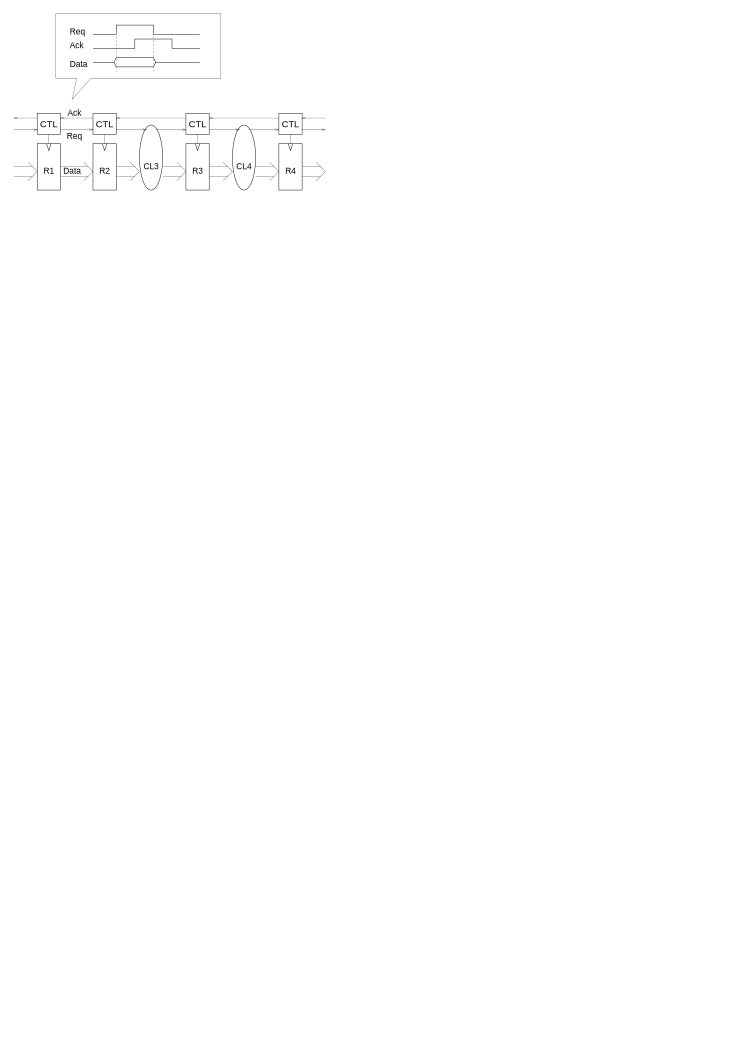
\includegraphics{handshake.pdf}
  \caption{A clockless pipeline implemented with handshaking ensuring
    data validity. The channels are bundled data four phase push
    channels. Figure from \cite{sparso}.}
  \label{fig:handshake}
\end{figure}

To connect and synchronize blocks in a clockless circuits, a form of
handshaking is usually employed, often as a request-acknowledge
protocol shown in figure~\ref{fig:handshake}. The handshaking provides
a local clock for the storage elements, usually latches or C-elements.

There are multiple ways to implement handshaking. Some high level
synthesis tools, introduced in section~\ref{sec:tools}, allow the
designer to choose and evaluate multiple implementation styles. The
Tangram/Haste synthesis tool allows handshake circuits to be
implemented as clocked circuits, making verification on regular FPGAs
\nomenclature{FPGA}{Field-Programmable Gate-Array} possible.

\subsection{Encodings}

Clocked digital circuits often use regular binary encoding where one
wire corresponds to one bit; a high voltage corresponds to a 1 and a
low voltage to a 0. While this encoding is possible with clockless
circuits, it has the drawback of not indicating completion. Other
encodings, discussed below, can also provide completion detection, an
important property of a QDI design. Choice of encodings has also been
shown to have significant impact on power.
 
\begin{figure}[htbp]
  \centering
  \includegraphics{bundled.pdf}
  \caption{An abstract view of a channel with bundled data, and two
    different protocols for data validity. Figure from \cite{sparso}.}
  \label{fig:bundled}
\end{figure}

When using bundled data, values are represented by conventional
boolean levels, and the handshaking is implemented by bundling request
and acknowledge signals with data as shown in
figure~\ref{fig:bundled}~a). Bundled data is also referred to as
single rail, in contrast to e.g. dual rail encoding, as data is
encoded as ordinary binary data. Usually there is no way to determine
whether binary data from a combinational function is complete, delays
matching the combinational delay in the critical path have to be
inserted in the control path to maintain correct behaviour.

\begin{table}
  \centering
  \begin{tabular}{|c|c|}
    \hline
    \emph{Electrical signal} & \emph{Interpretation} \\
    \hline
    0 0 & ``NULL''; no value \\
    0 1 & false, 0 \\
    1 0 & true, 1 \\
    1 1 & invalid \\
    \hline
  \end{tabular}
  \label{tab:dr}
  \caption{Dual rail representation of a boolean value.}
\end{table}

If the signal is encoded into a representation using two wires per
bit, one for each value; logic 1 (true) and logic 0 (false), it is
possible to distinguish successive values by seperating them with an
``empty'' value, also referred to as a ``NULL''. This encoding is
referred to as ``dual rail'' encoding, and is summarized in
table~\ref{tab:dr}.

\begin{figure}[htbp]
  \centering
  \includegraphics{drgate.pdf}
  \caption{a) A dual rail inverter. b) A strongly indicating dual rail
    and-gate, and c) the simulated and-gate. Note that the output is
    not showing a value until both inputs does, and that the value is
    held until \emph{both} inputs are returned to ``NULL''.}
  \label{fig:drgate}
\end{figure}

When implementing combinational functions for dual rail encoding, they
are typically split into two functions analogous to the pull up and
pull down networks in CMOS; one to compute the logic 0 or false value,
and one to compute the logic 1 or true value. A dual rail gate
implementation illustrating this is shown in figure~\ref{fig:drgate},
where one C-element is used to calculate a 1, and the other gates are
used to calculate a 0. Dual rail gates can often be less complex than
the example, by combining and optimizing the gates. While the and-gate
implementation shown in figure~\ref{fig:drgate} is state-holding, and
holds a calculated value until all (both) inputs returns to NULL, not
all gates need to have such complicated implementations. Usually, the
double area is needed to implement a dual-rail circuit over that of
single-rail.

A more generalized method for encoding is N of M encodings, where dual
rail is 1 of 2 encoding. All these encodings are constant-weight (N)
encodings, meaning that a complete signal has a certain hamming
weight, that is the count of electrical ones on a complete signal. In
\cite[chapter 9]{nullconv}, multiple of these encodings are surveyed
with regards to required resources (i.e. area) for wires and logic,
and power. An ALU for 1 of 4 encoding are shown to have good
characteristics in terms of power, area and performance, compared to
the dual rail encoding.

\subsection{Protocol}

When using handshake protocols, the handshake can be done in four or
two phases as shown in figure~\ref{fig:bundled}~b) and c). The four
phase protocol is also referred to as return to zero (RTZ). The two
phase protocol makes better use of the bandwith over the wires, but
usually the four phase protocol is preferred, as it allows for a
simpler implementation consuming less area.

In figure~\ref{fig:bundled}~a), a \emph{push} channel is shown. This
means that the data source initiates the handshake with the request
signal, as opposed to when the receiver inititates it. A channel where
the receiver initiates the handshake is referred to as a \emph{pull}
channel.

\begin{figure}[htbp]
  \centering
  \includegraphics{compdet.pdf}
  \caption{A memory element for dual-rail implementations with
    completion detection. Figure from \cite[pp. 21]{sparso}.}
  \label{fig:compdet}
\end{figure}

In the case of QDI (e.g. dual-rail) encodings, completion detection
provides either the request or acknowledge signal. Completion is
detected by counting the number of electrical ones, as shown in
figure~\ref{fig:compdet}, providing either a request signal in the
case of a push channel, or an acknowledge signal in the case of a pull
channel. The completion detector in figure~\ref{fig:compdet} provides
the request signal, and is therefore the receiver in a push channel.

Using dual rail encoding usually also implies using the four phase
protocol\footnote{For the sake of completeness, two phase protocol is
  possible with level-encoded two phase dual-rail (LEDR)\cite{ledr},
  but it is considered impractical for other uses than on long wires
  on chip.}  (figure~\ref{fig:bundled}~b)), as the combinational
circuits must return to the NULL state between values to distinguish
successive values on the channel. Care must therefore not only be
taken to avoid hazards on NULL-to-value transitions, but also on the
return-to-NULL transitions.


\subsection{Testing}

When producing integrated circuits, it is vital to ensure that the
defective ICs are removed from the production line as soon as
possible. Multiple defects can occur during modern fabrication that
can render ICs unusable or limit lifetime.

To determine which chips that are OK and not, testing must be
performed. Testing methods was divided into two categories by
\cite{eldred}: Functional testing, and structural testing.

In functional testing, the circuit is tested in its normal operation
mode, and no modifications to the circuit are needed. However, without
good knowledge of the underlying logic of a circuit under test, only
exhaustive testing can guarantee that the circuit will function for
all possible inputs. For e.g. a 32-bit adder, this means that $2^{64}
\approx 10^{19}$ vectors must be tested, which will, at an
unreasonable high test frequency of \unit{1}{\giga \hertz}, take
approximately \unit{10^{10}}{\second}, or 317 years to perform,
leaving functional testing unreasonable for this circuit.

Another form for functional testing, built in self test
(BIST\nomenclature{BIST}{Built-In Self Test}), utilizes e.g. an on
chip processor to test the functionality present on the chip, and can
also be used to determine the maximum safe operating speed of the
chip, as this test runs ``at speed''. An example of BIST is the
testing of RAM by writing and verifying all bits accessible. BIST is
possible to implement both on clocked and clockless circuits.

With structural testing, a \emph{fault model} is choosen to give a
simplified, but reasonable model of defects that can occur. Based on
the fault mode, test patterns are generated to cover the maximum
number of faults, that is inputs that will yield a wrong output in the
presence of a fault.

To design-for-test (DfT\nomenclature{DfT}{Design-for-Test}) is to
design hardware with modifications to make it more testable. More
complicated circuits than the mentioned 32 bit adder where inputs can
be controlled, and outputs observed, are circuits where inputs are
driven by e.g. internal registers, and where the outputs are not
directly observable. In such circuits, either arbitrarily long
sequences must be applied to steer and observe the registers, or test
points must be inserted.

With clocked circuits, such test points are usually implemented by
connecting multiplexers to registers, choosing whether the circuit
should operate in the normal mode, or that the registers should be
connected in series, making a scan-chain. Scan-chains are
shift-registers that make it possible to control and observe all the
scan-enabled registers. Scan-chains also allows single-stepping the
circuit, and by stopping the clock (and traditionally the entire
circuit), $I_{DDQ}$ tests can be performed to find shorts in the
circuit.

\begin{figure}[htbp]
  \centering
  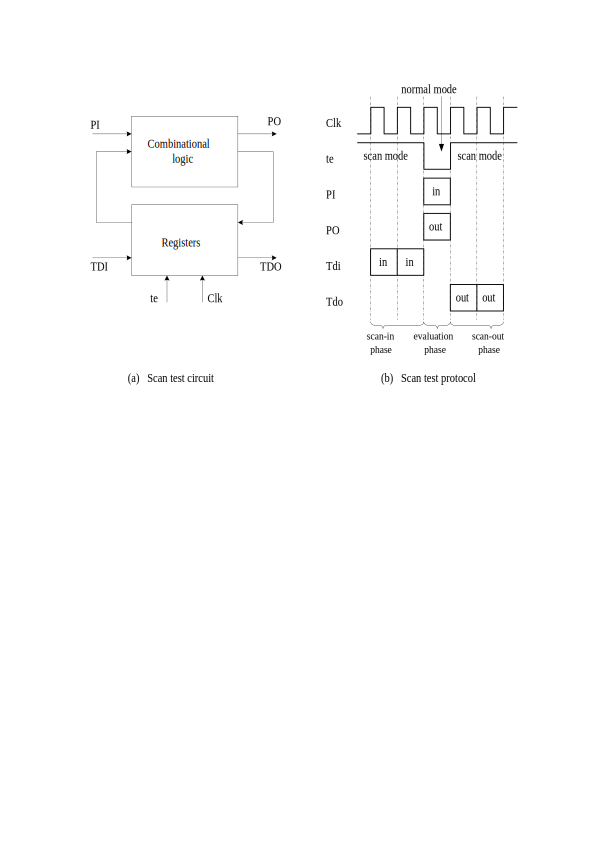
\includegraphics{scanint.pdf}
  \caption{a) A synchronous scan-interface, and b) protocol. Figure
    from \cite[pp. 11]{fullscan}.}
  \label{fig:scanint}
\end{figure}

Figure~\ref{fig:scanint} shows a typical scan-interface. This is
fairly standard, and equipment to interface with it is fairly
standard, and considered an industry standard. Therefore, it is
a good idea to implement the same interface for testing for clockless
circuit, to make it a more attractive method of producing circuits.

In \cite[pp. 27-28]{sparso} testing of clockless circuits is briefly
discussed, noting that the indication-principle will cause a circuit
with a stuck-at fault to deadlock. In \cite[pp. 26]{fullscan}, this is
referred to as the ``acknowledge property'', and it is noted that this
only holds for the practical unuseful class of delay-insensitive
circuits. In the more applicable quasi delay insensitive kind of
circuits, isochronic forks can extend faults to not only cause a
circuit to deadlock, but also lead to a misbehaving circuit.
Furthermore, \cite{fullscan} provides methods for implementing a
synchronous scan-interface to clockless circuits are introduced and
tested.

\subsection{Initialization and reset}

A clocked circuit is usually started by asserting a reset signal to
put it in a defined state,and then releasing the reset signal to let
the circuit start operating. The reset signal is either said to be
synchronous or asynchronous with regards to the global clock. A
synchronous reset signal must, as other signals, arrive within the
setup and hold times of the flip flops. An asynchronous reset must be
released simultaneously across the whole circuit, a problem which is
as hard as distributing a global clock.

Not all parts of a circuit usually need to be set in a known state
for a circuit to operate correctly. E.g. a circuit that receives some
input into registers, processes the data, and then outputs the
results, need not to reset the data-registers as they will be
overwritten before the register content is used in the calculations.

Clockless circuits also need initialization, but based on the
read-after-write principle illustrated above, in principle only the
top-most control circuit needs initialization, which then initializes
sub circuits with handshaking when needed. This method of
initialization is generally used in handshake circuits described
in~\ref{sec:tools} on page~\pageref{par:init}.

